\chapter{Introduction}\label{sec:introduction}

According to the latest Cisco's VNI \cite{video-traffic-forecast}, video will
account for 82\% of all IP traffic in Europe by 2021; in addition, the overall IP
traffic per person will triplicate from 13\emph{GB} to 35\emph{GB}. These
forecasts clearly picture the growth of the streaming industry, posing, at the
same time an important question on the present and future states of the final
user's privacy.

As shown by Reed et Al. \cite{netflix-real-time} anonimity of user's viewing
activity is at risk. Not for the use that Netflix or other streaming services
do of user's session data, but because of the risk of a man-in-the-middle
attack \emph{MITM} carried by an \textit{evil} party. 

In particular, they have shown how the adoption of HTTPS to protect video
streams from Netflix \emph{CDN}s to user's end devices, does not hold against
passive traffic analysis.

\section{Motivation}\label{motivation}

The goal of this project is to replicate part of the work conducted by Reed et
Al. and to investigate the possibility of identifying a Netflix stream solely
based on the observed average bandwidth. This, follows from the intuition that
\emph{per-title encoding} embeds the nature and the complexity of video frames
in a unique way, that may reveal the identity of the content being streamed.

\subsection{Per-Title Encoding}\label{sec:per-title-encoding}

In December 2015 Netflix announced \cite{per-title-encoding} that it was
introducing a new method to analyze the complexity of each title and find the
best encoding recipe based on it. Their goal with the adoption of
per-title encoding was to provide users with better quality streams at a lower
bandwidth. 

Before then, each title was encoded with a \emph{Fixed Bitrate Ladder}; their
pipeline returned a list of \{\emph{Bitrate, Resolution}\} pairs that
represented the sufficient bitrate to encode the stream at a certain
resolution (\Cref{tab:fixed-ladder}), with no visible artificats.

\begin{table}[htb]
  \centering
  \begin{tabular}{|c|c|}
    \hline
    \textbf{Bitrate (kbps)} & \textbf{Resolution} \\
    \hline
    235                     &    $320\times240$ \\
    \hline
    375                     &    $384\times288$ \\
    \hline
    560                     &    $512\times384$ \\
    \hline
    750                     &    $512\times384$ \\
    \hline
    1050                    &    $640\times480$ \\
    \hline
    1750                    &    $720\times480$ \\
    \hline
    2350                    &   $1280\times720$ \\
    \hline
    3000                    &   $1280\times720$ \\
    \hline
    4300                    &   $1920\times1080$ \\
    \hline
    5800                    &   $1920\times1080$ \\
    \hline
  \end{tabular}
  \caption{Netflix original's Fixed Bitrate Ladder}
  %\end{center}
  \label{tab:fixed-ladder}
\end{table}

This "one-size-fits-all" ladder, as reported, achieved good results in the
encoded video's perceived quality (\textbf{PSNR} \cite{psnr}) given the bitrate
constraint, but, would not perform optimally under certain conditions. For
instance, high detailed scenes with sudden changes of light, or rapid
transitions of camera shots, would require more than 5800\emph{kbps}; in
contrast, more static frames, as in animated cartoons, may be encoded at higher
resolutions mantaining the same bitrate level.

In summary they noticed how in certain cases, the produced encoding would
either present some small artifacts (\emph{e.g.} complex scenes), or waste
bandwidth, (\emph{e.g.} static, plain scenes). For this reason, they came up
with per-title encoding.

\begin{table}[htb]
  %\begin{center}
  \centering
  \begin{tabular}{|c|c|c|}
    \hline
    \textbf{Resolutions} & \textbf{Fixed Bitrate Ladder (kpbs)} & \textbf{Per-Title Bitrate Ladder (kbps)} \\
    \hline
    $320\times240$       & 235                                  & 150 \\
    \hline
    $384\times288$       & 375                                  & 200 \\
    \hline
    $512\times384$       & 560                                  & 290 \\
    \hline
    $512\times384$       & 750                                  & \\
    \hline
    $640\times480$       & 1050                                 & \\
    \hline
    $720\times480$       & 1750                                 & 440\\
    \hline
    $720\times480$       &                                      & 590\\
    \hline
    $1280\times720$      & 2350                                 & 830\\
    \hline
    $1920\times1080$     & 3000                                 & 1150\\
    \hline
    $1920\times1080$     & 4300                                 & 1470\\
    \hline
    $1920\times1080$     & 5800                                 & 2150\\
    \hline
    $1920\times1080$     &                                      & 3840\\
    \hline
  \end{tabular}
  \caption{
    Comparison between the two different approaches for the same title: note
    how different titles may have different numbers of quality levels. For each
    movie, the minimum number of quality levels gets computed to produce a
    just-noticeable-difference (JND), when switching bitrates during playback.
  }
  \label{tab:old-vs-new-ladder}
\end{table}

In order to find the best fitting bitrate ladder for a particular title, there
are several criterias that they took into account, the principal ones being:

\begin{itemize}
    \item How many quality levels should be encoded to obtain a
          \emph{JND} between each of them.
    \item Best \{\emph{Resolution, Bitrate}\} pair for each quality level
    \item Highest bitrate required to achieve the best perceivable quality
\end{itemize}

As aforementioned, each title's perceived video quality, gets computed as a
measure of \emph{Peak signal-to-noise ratio}. The comparison is performed
between the produced encode, upsampled to 1080\emph{p}, and the original title
in 1080\emph{p}, and the best \{\emph{Bitrate, Resolution}\} pair is assigned
to that specific quality level, as depicted in \Cref{tab:old-vs-new-ladder}.

In \Cref{fig:new-vs-old-ladder}, we can see the impact of per-title encoding on
the original bitrate ladder: in order to achieve the same perceivable quality
level (point \textbf{B} and \textbf{C}), it requires a lower bitrate to be
encoded to (point \textbf{A}).  Moreover, with around the same bitrate, one can
see how per-title encoding can achieve a higher resolution compared the fixed
case (point \textbf{A} and \textbf{D} respectively). It follows obviously that,
holding to a high-quality stream while maintainig or lowering the used
bandwidth is key: the end user will get same or better quality then before, at
a lower bandwidth.

\begin{figure}[htb]
  \centering
  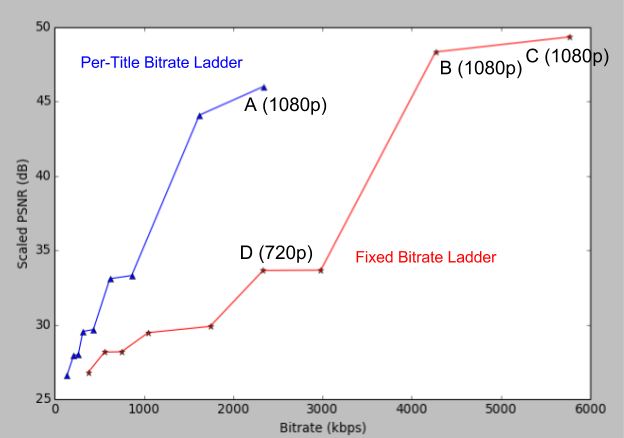
\includegraphics[width=0.9\columnwidth]{img/pertitlevsfixed.png}
  \caption{Difference between per-title vs. fixed bitrate ladders}
  \label{fig:new-vs-old-ladder}
\end{figure}

\subsection{User's Privacy}\label{sec:privacy}

%TODO add privacy concerns, explain who\why and how can collect/make use of 
%this data. 

\section{Related Work}\label{related}

%TODO add previous work section

%TODO Reed et Al. 2017
%TODO Saponas devices 2007
%TODO Moser ETH BSc thesis 2018

\section{Main Objective}\label{sec:objective}

%TODO What is the goal of the project?

\section{Structure of this Report}\label{sec:structure}

%TODO briefly summarize how we want to develope our discourse during each chapter

%TODO Chapter 1 - Introduction [THIS]
%TODO Chapter 2 - End to End Attack Scenario 
               %- Describe the attack scenario from the perspective of an ISP
               %- Describe the infrastructure
               %- Describe what kind of information the attacker is able to retrieve
               %- Outlie the consequences of such an attack
%TODO Chapter 3 - Approach
               %- Present our version of the attack scenario
               %- Describe the infrastructure
               %- Present the data we have collected
               %- Highlight the differences from our approach to Reed's et Al.
               %- Explain how we can uniquely identify a movie / Explain how we
                  %make use of the features we collect
%TODO Chapter 4 - Evaluation of the system
               %- Explain Plots & result data
%TODO Chapter 5 - Conclusion
               %- Future Work
               %- Acknowlegments
